
\begin{center}
\textbf{Autodesk Inventor}
\end{center}
	\section{Softwares de CAD}
\subsection{Introdução}

	O Design mec\^anico atrav\'es de softwares CAD ({\it Computer Aided Design}, ou Design Auxiliado por Computador) \'e de suma import\^ancia ao projetar qualquer tipo de rob\^o, pois tendo em vista que toda a eletr\^onica deste ser\'a montada sobre a estrutura f\'isica do aut\^omato, \'e indispens\'avel que esta atenda todos os requisitos previamente decididos.
	
	Os softwares de CAD podem ser: Param\'etricos ou ???????. Para o nosso prop\'osito, o mais interessante \'e o param\'trico, pois permite uma gest\~ao precisa das depend\^encias entre os par\^ametros das pe\c{}as presentes no modelo.
	
	Os dois softwares mais populares neste segmento s\~ao o "SolidWorks", da Dassault Systemes, e o "Autodesk Inventor", da pr\'opria Autodesk. Ambos possuem interface e enfoque parecidos, mas cada um com suas particularidades. A opç\~ao de escolha entre um ou outro cabe apenas ao usu\'ario, tendo em vista que s\~ao softwares igualmente poderosos.
	Ainda, e\' digno de men\c{c}\~ao o "Solid Edge", da Siemens AG.
	\\
	\subsection{CAD Param\'etrico}
	
	Os softwares de CAD  param\'etrico nos possibilitam, atrav\'es das suas {\it features}, transformar um desenho 2D em um modelo 3D. Isso acontece desenhando, incialmente, um esbo\c{c}o da superf\'icie principal do modelo. Com este pronto, podemos adicionar a terceira dimens\~ao do modelo atrav\'es de recursos como a Extrus\~ao, que d\'a profundidade ao esboço ou a Revolu\c{c}\~ao, que revoluciona o esbo\c{c}o em torno de uma das suas laterais, criando uma esp\'ecie de cilindro.


	\begin{figure}[h]
	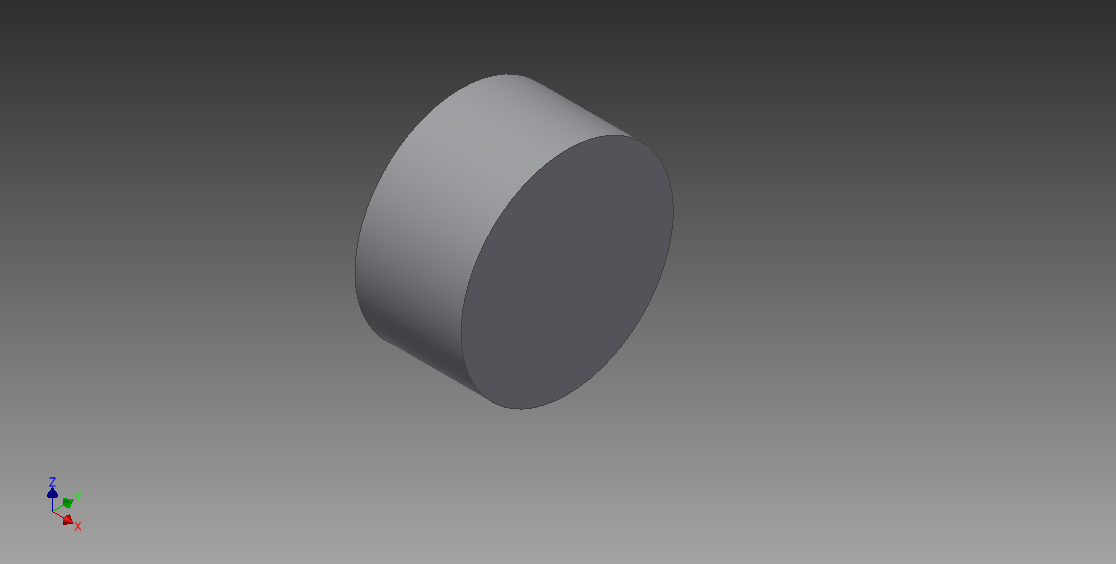
\includegraphics[scale=0.3]{./include/chapters/sections/mec/section1/imgs/box.png}
	\caption{Superf\'icie Revolucionada}
	\label{Rev}
	\end{figure}

	\begin{figure}[h]
	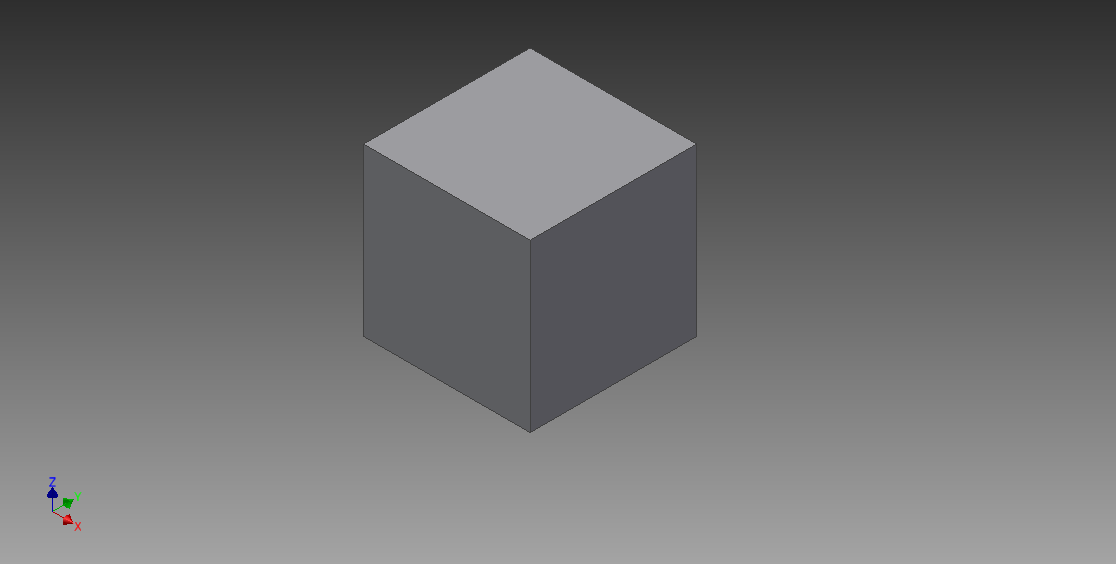
\includegraphics[scale=0.3]{./include/chapters/sections/mec/section1/imgs/rev.png}
	\caption{Superf\'icie Extrudada}
	\label{Ext}
	\end{figure}
\newpage
\section{Autodesk Inventor}

\subsection{Intro}

	O Autodesk Inventor teve a sua primeira edi\c{c}\~ao lançada em 1999 e desde ent\~ao tem se tornado uma das refer\^encias no segmento de CADs 3D. As suas fun\c{c}\~oes são in\'umeras, desde o desenvolvimento de modelos em 3D, at\'e o teste de materiais e constru\c{c}\~ao de apresenta\c{c}\~oes.

\subsection{Primeiras impressões - Autodesk Inventor Professional 2014}

A interface do Autodesk Inventor e\' muito semelhante  \`a dos seus concorrentes, com atalhos para as principais funç\~oes e recursos do software em uma barra superior, devidamente organizada entre r\'otulos. Um dos pontos positivos em rela\c{c}\~ao aos outros s\~ao os seus v\'arios tutoriais, que tornam o  software mais {\it user-friendly}, principalmente para "marinheiros de primeira viagem" no mundo do CAD.
\\	

\subsection{Criando um projeto}

	Ao clicar no \'icone "New", na tela inicial do software, uma janela chamada  ``{\it Create New File}" é aberta. Nesta, possu\'imos toda a gama de op\c{c}\~oes de projetos que o Autodesk Inventor \'e capaz de desenvolver. \'E interessante frisar que e\' aqui que ser\'a escolhida a unidade de medida do projeto, seja ela Imperial ({\it English}), ou M\'etrica ({\it Metric}).
	
	\begin{figure}[h]
	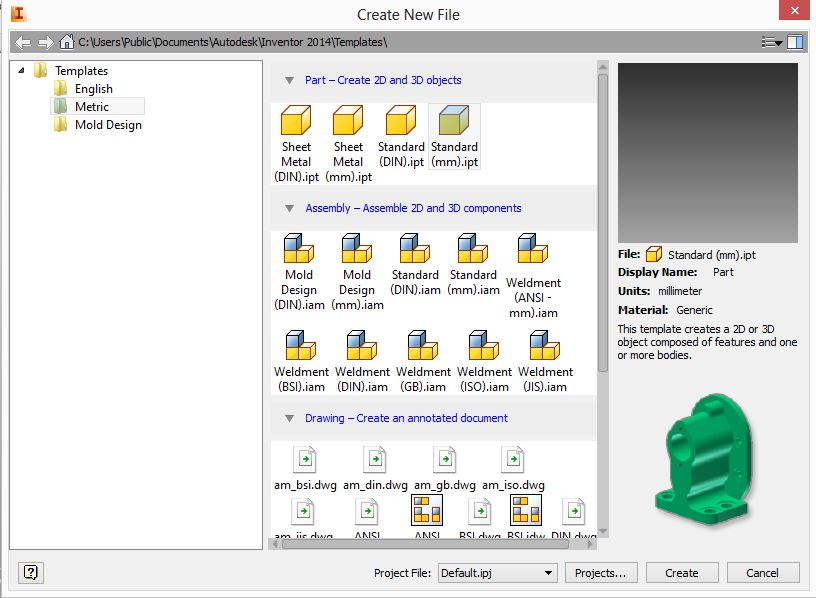
\includegraphics[scale=0.5]{./include/chapters/sections/mec/section1/imgs/first_wdw.jpg}
	\caption{Janela Create New File}
	\label{CreateNew}
	\end{figure}
\newpage
	Na parte superior da tela seguinte, encontramos toda a sorte de opç\~oes e recursos implement\'aveis nos esbo\c{c}os e desenhos desenvolvidos no software.
	\\
	\begin{figure}[h]
	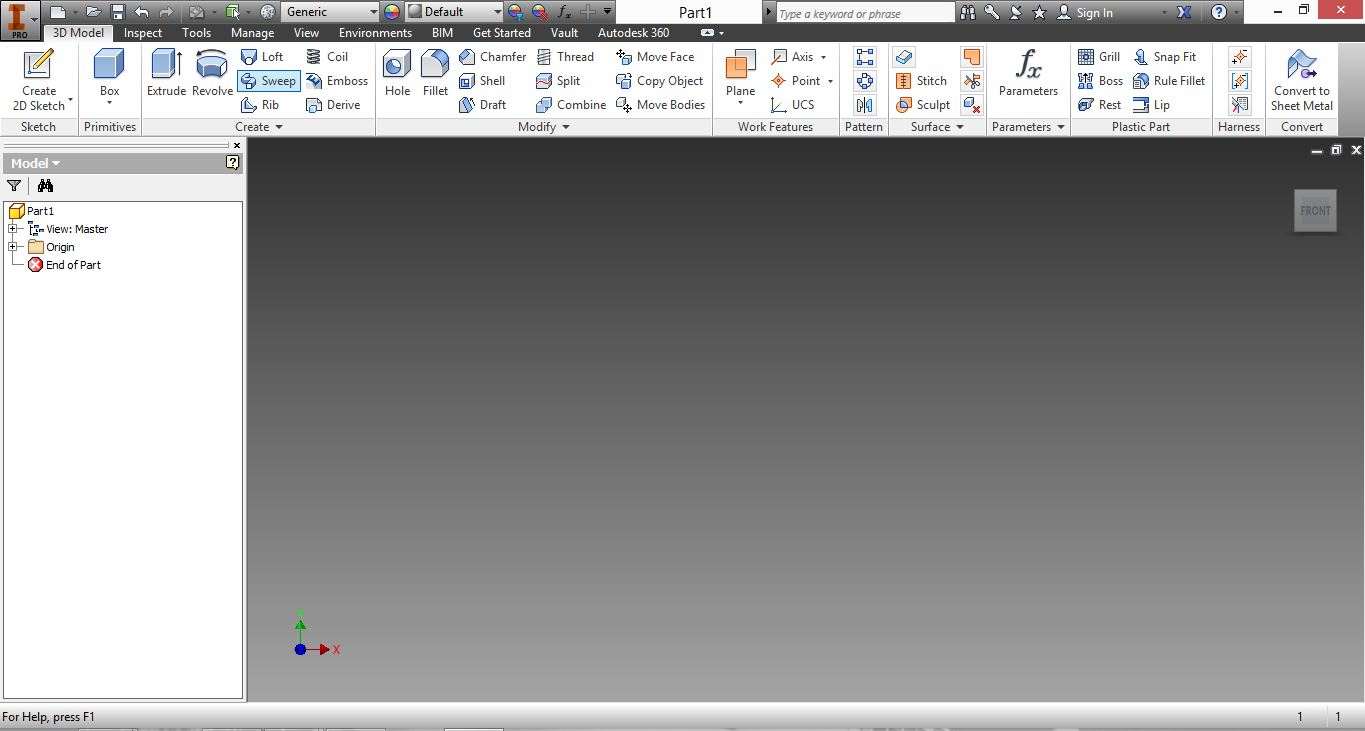
\includegraphics[scale=0.3]{./include/chapters/sections/mec/section1/imgs/sec.jpg}
	\caption{Primeira \'Area de Trabalho}
	\label{Desktop}
	\end{figure}
	\\
\subsection{Criando o desenho em 2D (Desenho T\'ecnico)}

	Outro recurso muito interessante do Autodesk Inventor e\' a possibilidade de criar um desenho em 2D cotado em v\'arios \^angulos (Desenho T\'ecnico) \`a partir de um modelo 3D. Essa op\c{c}\~ao est\'a dispon\'ivel na janela acima citada ``{\it Create New}", na se\c{c}\~ao ``{\it Drawing}". 
	\\
	Ap\'os escolhido o padr\~ao da folha de desenho t\'ecnico, os passos seguintes s\~ao bem instintivos, auxiliados por uma caixa de op\c{c}\~oes.
	
	\begin{figure}[h]
	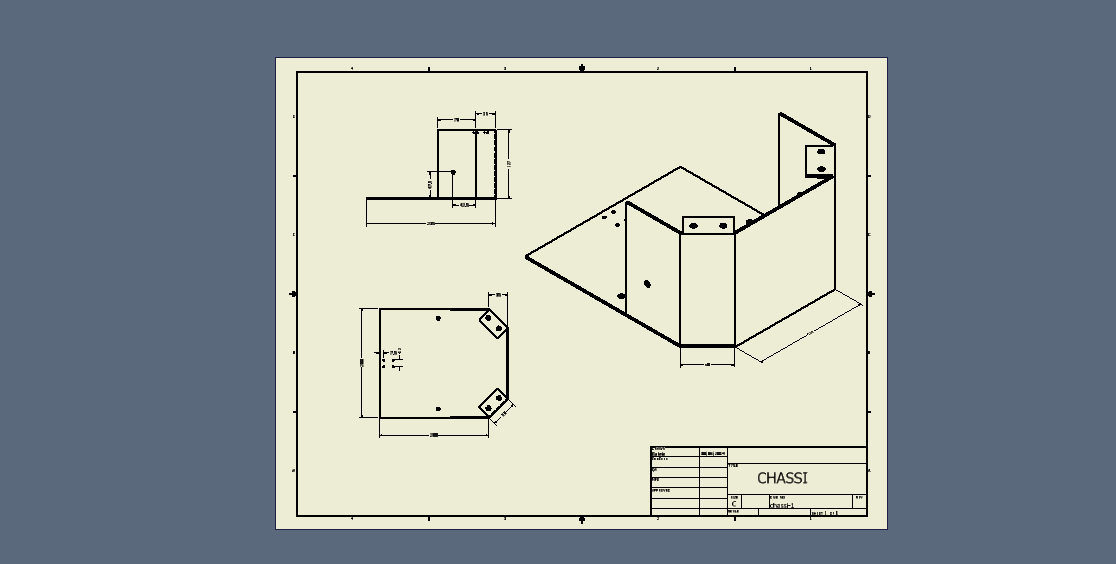
\includegraphics[scale=0.5]{./include/chapters/sections/mec/section1/imgs/chassi.png}
	\caption{Exemplo de Drawing}
	\label{Chassi}
	\end{figure}
\newpage
\subsection{Vista Explodida}

	Um recurso muito \'util do Autodesk Inventor e\' a possibilidade de criar a vista explodida de uma montagem (ou ``{\it Assembly}" ), \`a partir de um modelo criado previamente atrav\'es do software. Ainda, podemos criar uma anima\c{c}\~ao de montagem ou desmontagem do modelo com este mesmo recurso.
	
	Para utiliz\'a-lo, deve-se, novamente, ir \`a janela ``\textit{Create new}" e ali escolher o Item ``\textit{Presentation}".
	
	Tendo escolhido tamb\'em o padr\~ao da apresentaç\~ao, uma nova a\'rea de trabalho ser\'a aberta. Nesta, devemos escolher, inicialmente, a op\c{c}\~ao ``\textit {Create View}"  e checar a op\c{c}\~ao ``\textit {Manual}", pois desejamos construir a vis\~ao explodida manualmente (e porque o modo autom\'atico \'e ca\'otico).
	
	Na tela seguinte, acontece a "explos\~ao" pr\'opriamente dita, onde ao selecionar uma peça da ``\textit{Assembly} " clicamos em ``\textit{Tweak Component}" e escolhemos a dire\c{c}\~ao na qual desejamos levar a peça na vista explodida.
	\\
	\begin{figure}[h]
	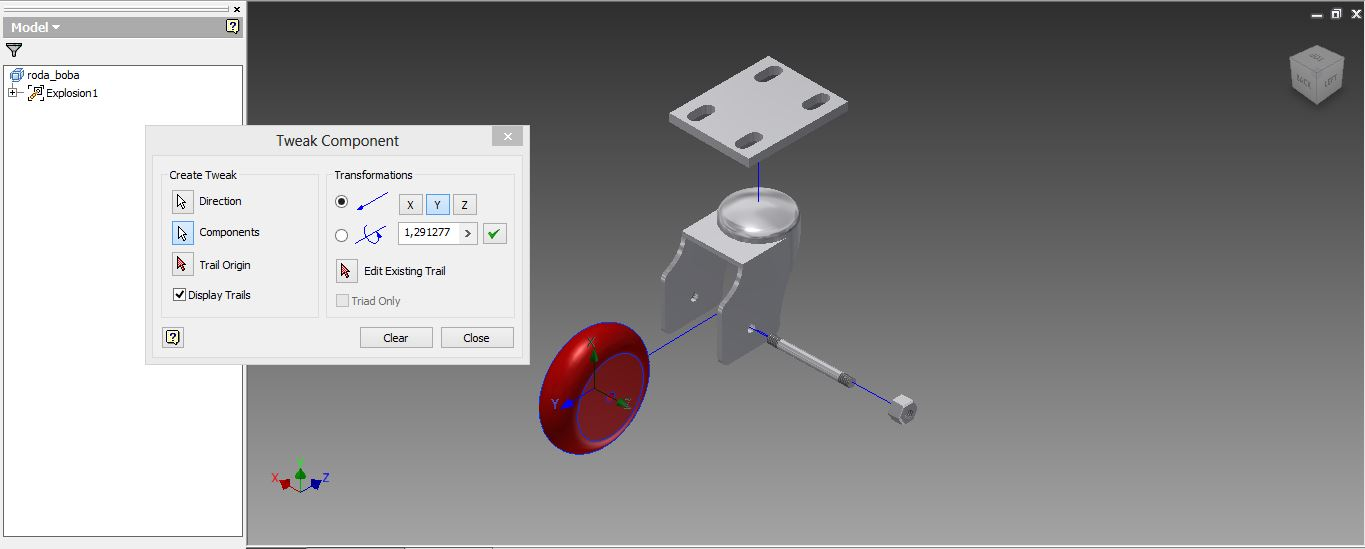
\includegraphics[scale=0.3]{./include/chapters/sections/mec/section1/imgs/exp.jpg}
	\caption{Constru\c{c}\~ao da Vista Explodida}
	\label{Chass}
	\end{figure}
